\textbf{ProductCategoryList}

ProductCategoryList er en ObservableCollection<ProductCategory>~\cite{ObsCol}, som indholder de sidst hentede ProductCategorier fra \gls{CS}. Når Update() kaldes opdatere ProductCategoryList sig selv ved at hente alle ProductCateogies fra \gls{CS} via DBcontrol, og overskriver sin ObservableCollection med disse.\\
Grunden til at ProductCategoryList ikke er lavet som en ViewModel, er at knapperne med produkterne kræver lidt mere behandling grundet buttonpages. ProductCategoryList, er derfor en Model, som præsentere produkterne op til ProductButtonControl.

\begin{figure}[H]
    \centering
    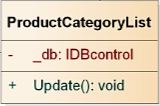
\includegraphics[width=30mm]{Systemdesign/Frontend/BLL/Pics/ProductCategoryList}
    \caption{ProductCategoryList}
    \label{fig:ProductCategoryList}
\end{figure}

\bigskip